\documentclass[aspectratio=169,11pt]{beamer}

\usetheme{Boadilla}
\usecolortheme{dolphin}

\usepackage[T1]{fontenc}
\usepackage[utf8]{inputenc}
\usepackage{booktabs}
\usepackage{graphicx}
\usepackage{hyperref}
\usepackage{tikz}
\usetikzlibrary{arrows.meta,positioning}

\title[Witsmith]{Witsmith}
\subtitle{The contract your coding agent did not know it needed}
\author{Team Witsmith}
\institute{Cursor Hackathon}
\date{\today}

\hypersetup{
  pdftitle={Witsmith pitch deck},
  pdfauthor={Team Witsmith},
  colorlinks=true,
  urlcolor=blue
}

\setbeamertemplate{navigation symbols}{}
\setbeamertemplate{footline}[frame number]

% Set to \showappendixtrue if you want the playbook backup slides in the PDF.
\newif\ifshowappendix
\showappendixfalse

\newcommand{\assetorbox}[3]{%
  \IfFileExists{#1}{%
    \includegraphics[width=#2\linewidth,height=.68\textheight,keepaspectratio]{#1}%
  }{%
    \begin{center}
      \fbox{%
        \begin{minipage}[c][.58\textheight][c]{#2\linewidth}
          \centering
          \Large #3\\[1ex]
          \normalsize Replace with \texttt{#1}
        \end{minipage}%
      }
    \end{center}
  }%
}

\begin{document}

\begin{frame}
  \titlepage
  \vfill
  \centering
  \Large Your agent just got prompt-injected. Witsmith caught it, rolled it back, and patched its own permission file.
\end{frame}

\begin{frame}{Meet Smith}
  % Image path must match the file on disk exactly (e.g. no leading space in the filename).
  \assetorbox{assets/smith.png}{.86}{Sheepish Smith + \texttt{.env}}

  \vfill
  \centering
  Smith reads every file in the repo, including the ones with instructions in them.
\end{frame}

\begin{frame}{The Loop}
  \IfFileExists{assets/loop.png}{%
    \centering
    \includegraphics[width=.96\linewidth,height=.66\textheight,keepaspectratio]{assets/loop.png}
  }{%
    \centering
    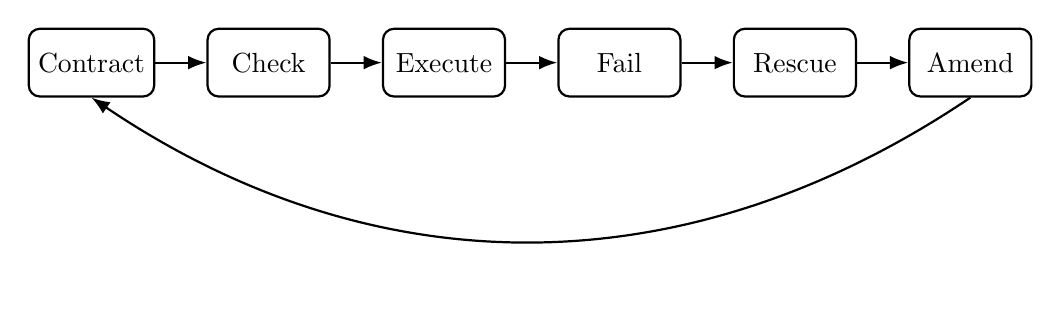
\begin{tikzpicture}[
      node distance=.65cm,
      every node/.style={draw, rounded corners, align=center, minimum width=1.55cm, minimum height=.86cm},
      every path/.style={-Latex, thick}
    ]
      \node (contract) {Contract};
      \node[right=of contract] (check) {Check};
      \node[right=of check] (execute) {Execute};
      \node[right=of execute] (fail) {Fail};
      \node[right=of fail] (rescue) {Rescue};
      \node[right=of rescue] (amend) {Amend};

      \path (contract) edge (check);
      \path (check) edge (execute);
      \path (execute) edge (fail);
      \path (fail) edge (rescue);
      \path (rescue) edge (amend);
      \path (amend.south) edge[bend left=34] (contract.south);
    \end{tikzpicture}
  }

  \vfill
  \centering
  \small Contract $\rightarrow$ action $\rightarrow$ failure $\rightarrow$ recovery\\[.35ex]
  $\rightarrow$ amendment $\rightarrow$ contract.
\end{frame}

\begin{frame}{The Wow Moment}
  \IfFileExists{assets/wow-diff.png}{%
    \centering
    \includegraphics[width=.96\linewidth,height=.72\textheight,keepaspectratio]{assets/wow-diff.png}
  }{%
    \begin{block}{Live \texttt{AGENT\_WIT.yaml} diff}
      {\ttfamily\small
      ask:\\
      \hspace*{1em}- pattern: "rm -rf*"\\
      + - pattern: "*prisma migrate*"\\
      + \hspace*{1em}\# auto-added after Smith dropped users.email\\
      + \hspace*{1em}\# see .witsmith/handoffs/0042-smith-strikes-again.md
      }
    \end{block}
  }

  \vfill
  \centering
  Smith failed. The policy changed outside the agent. Smith cannot make the same mistake twice.
\end{frame}

\begin{frame}{Free Your Smith}
  \centering
  {\Huge Free your Smith.}

  \vspace{1.2cm}

  \begin{columns}[c]
    \begin{column}{.52\linewidth}
      \Large Witsmith is open source.\\[1ex]
      \normalsize Replace this with the final repo URL:\\
      \url{https://github.com/your-org/witsmith}
    \end{column}
    \begin{column}{.32\linewidth}
      \IfFileExists{assets/qr.png}{%
        \includegraphics[width=.9\linewidth]{assets/qr.png}
      }{%
        \fbox{\begin{minipage}[c][.32\textheight][c]{.9\linewidth}
          \centering QR code\\[1ex]
          \texttt{assets/qr.png}
        \end{minipage}}
      }
    \end{column}
  \end{columns}
\end{frame}

\ifshowappendix
\appendix

\begin{frame}{Problem: Static Permissions Miss New Failures}
  \begin{quote}
    ``AI coding agent deleted production database in 9 seconds.''
  \end{quote}

  \vfill
  \centering
  Replace this frame with a rights-safe incident quote or screenshot if you choose to show the playbook problem slide.
\end{frame}

\begin{frame}{What Is New}
  \centering
  \begin{tabular}{@{}lll@{}}
    \toprule
    Capability & Existing tools & Witsmith \\
    \midrule
    Hooks and allowlists & Yes & Yes \\
    Plan/act approvals & Yes & Yes \\
    Runtime amendment loop & No & Yes \\
    Natural-language source rules & No & Yes \\
    Prompt-injection headline demo & No & Yes \\
    \bottomrule
  \end{tabular}

  \vfill
  Static systems protect against failures you predicted. Witsmith learns from the ones you did not.
\end{frame}
\fi

\end{document}
